

\begin{figure}[h]
	\centering
	\subfloat[][\emph{$\rho$ and $SC_0$ dependence.}]
	{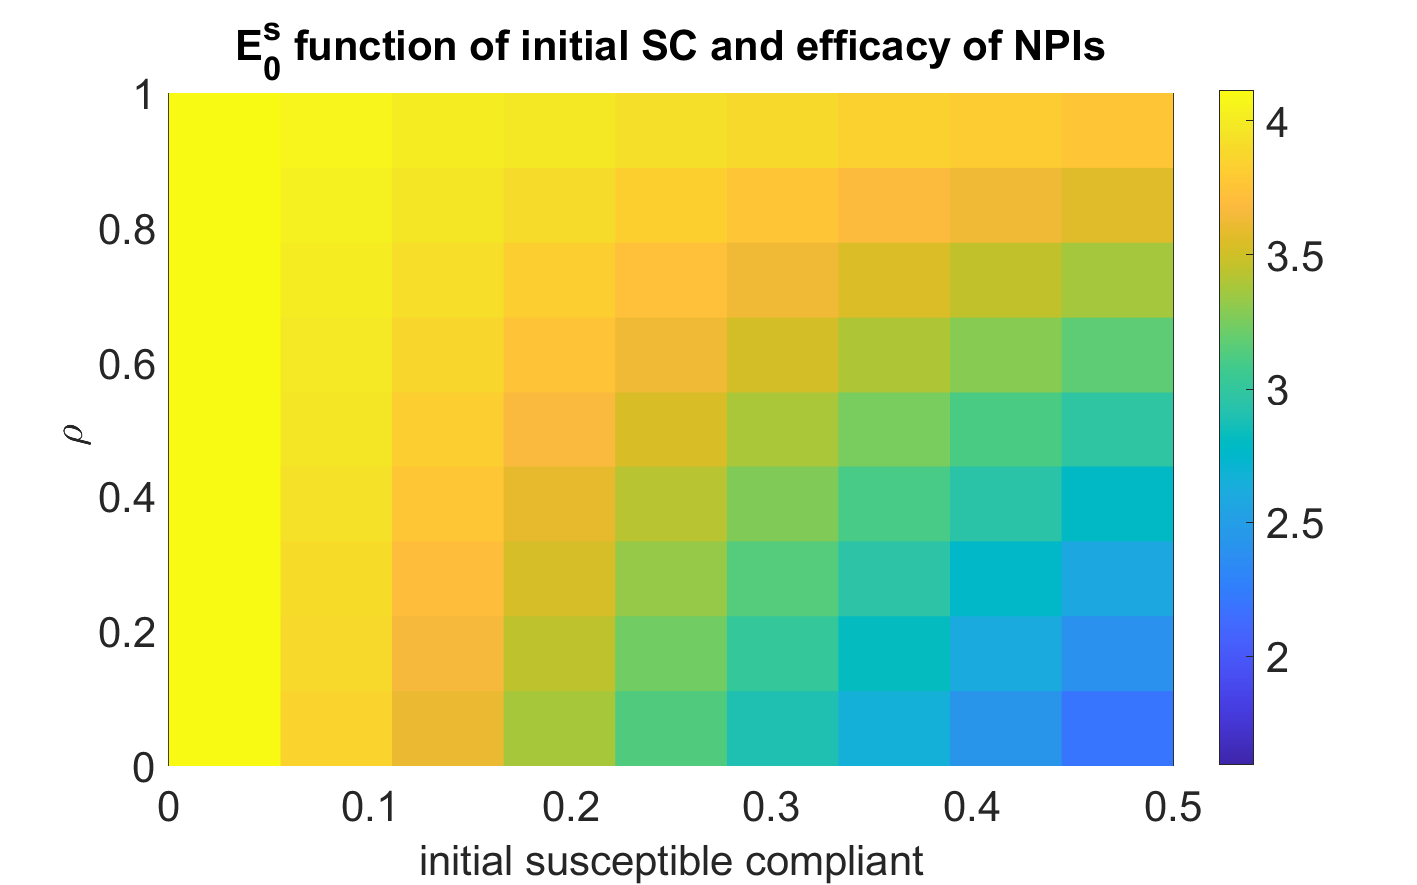
\includegraphics[width=0.48\linewidth]{1_corpo/figure/behav_epi_sim/HMap_SC0_rho_B1_B2_less_1}} \quad
	\subfloat[][\emph{ $SA_0$ and $SC_0$ dependence.}]
	{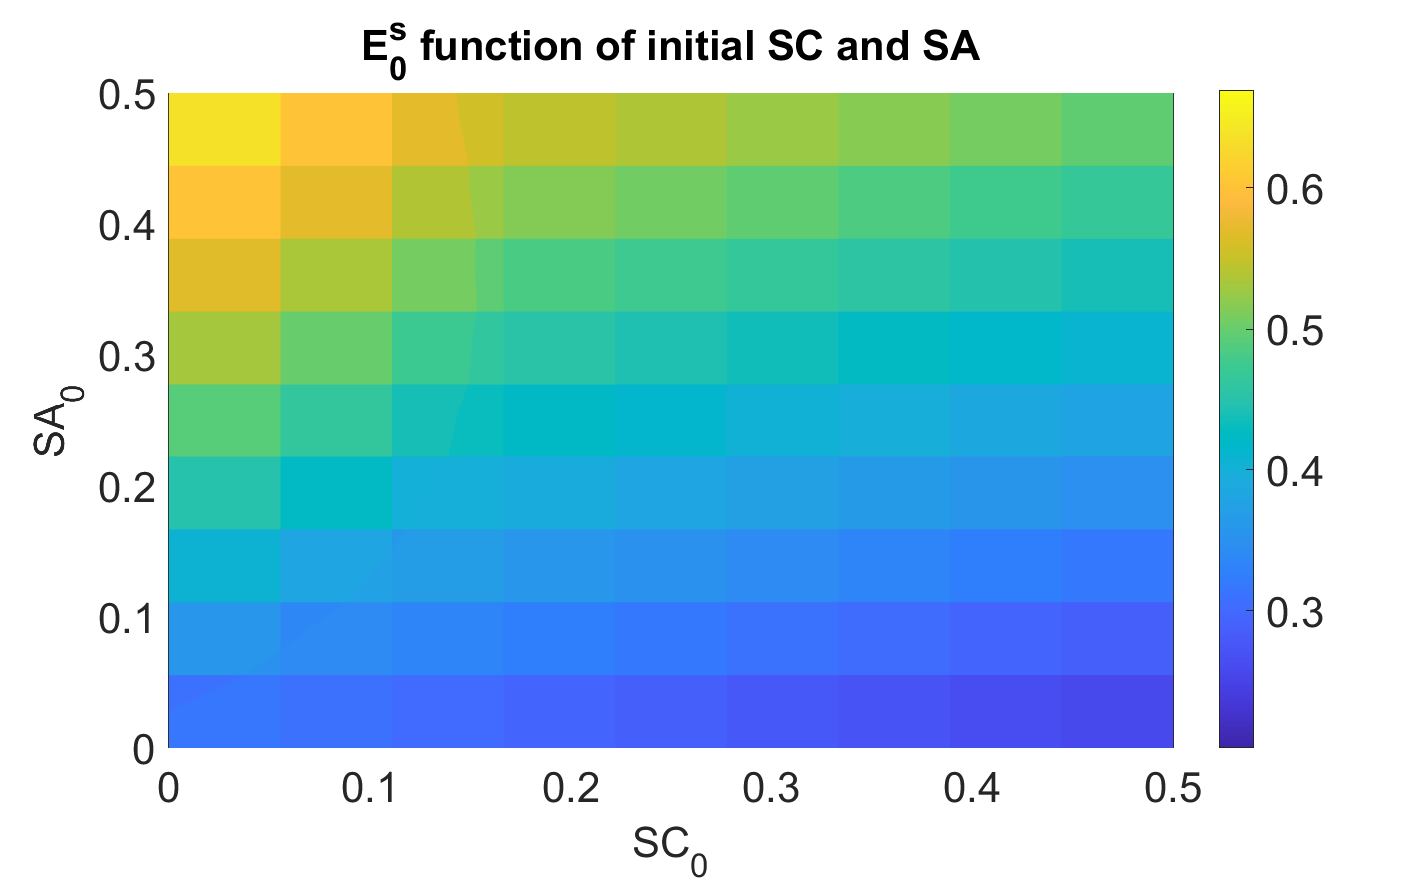
\includegraphics[width=0.48\linewidth]{1_corpo/figure/behav_epi_sim/HMap_SC0_SA0_B1_B2_less_1}}\\
	\caption[Heat map full model first case]{Simulations of $E_0^s$ with $\mathcal{B}_1, \mathcal{B}_2 <1$, $\mathcal{B}_1 >  \mathcal{B}_2$, and $\lambda_1 > \lambda_2$.}
	\label{fig:Hmap_B1_B2_less_1}
\end{figure}



\begin{figure}[h]
	\centering
	\subfloat[][\emph{$\rho$ and $SC_0$ dependence.}]
	{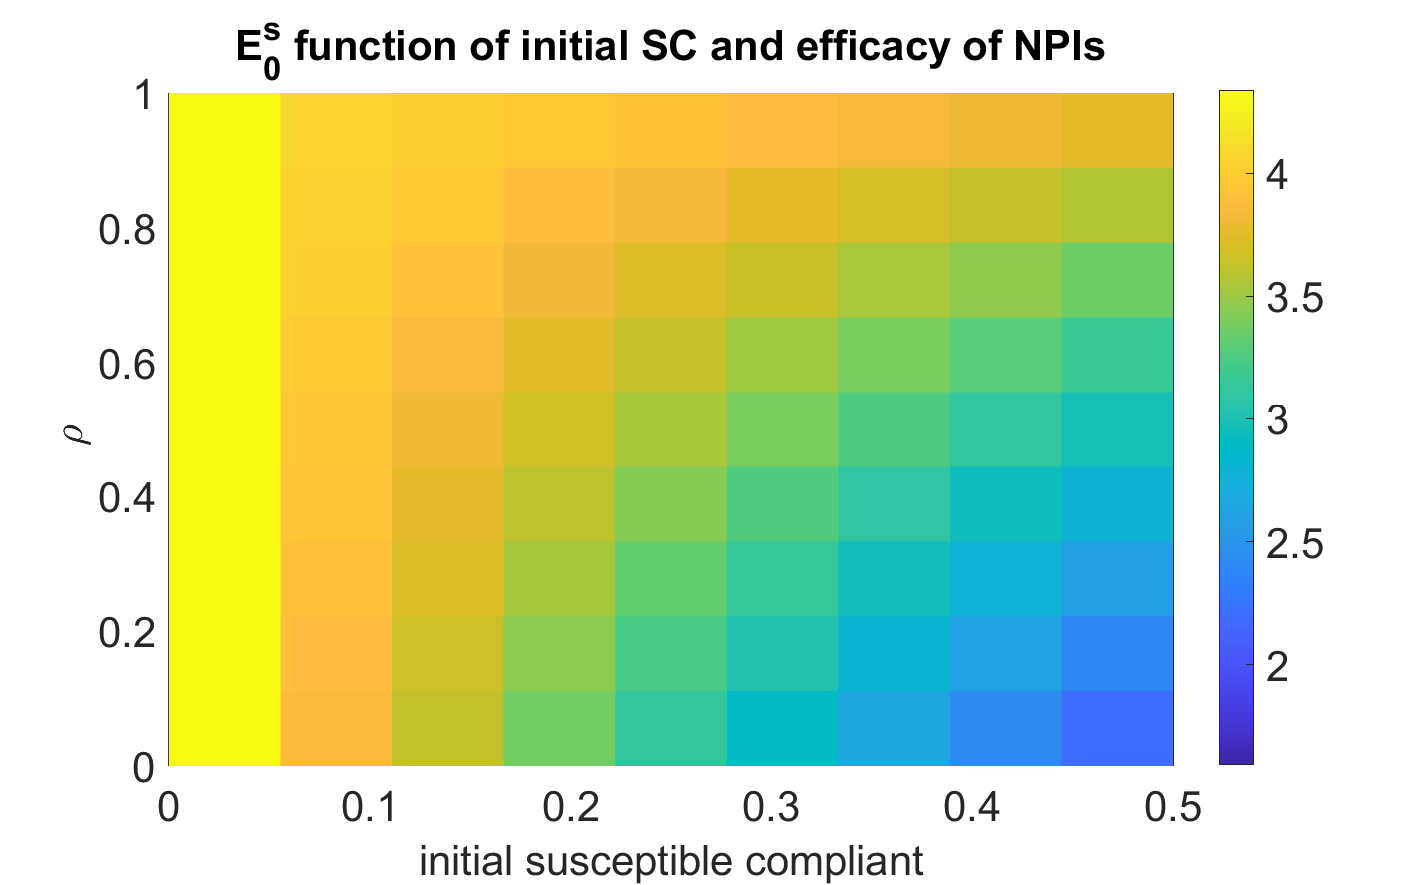
\includegraphics[width=0.48\linewidth]{1_corpo/figure/behav_epi_sim/HMap_SC0_rho_B1_B2_equal}} \quad
	\subfloat[][\emph{ $SA_0$ and $SC_0$ dependence.}]
	{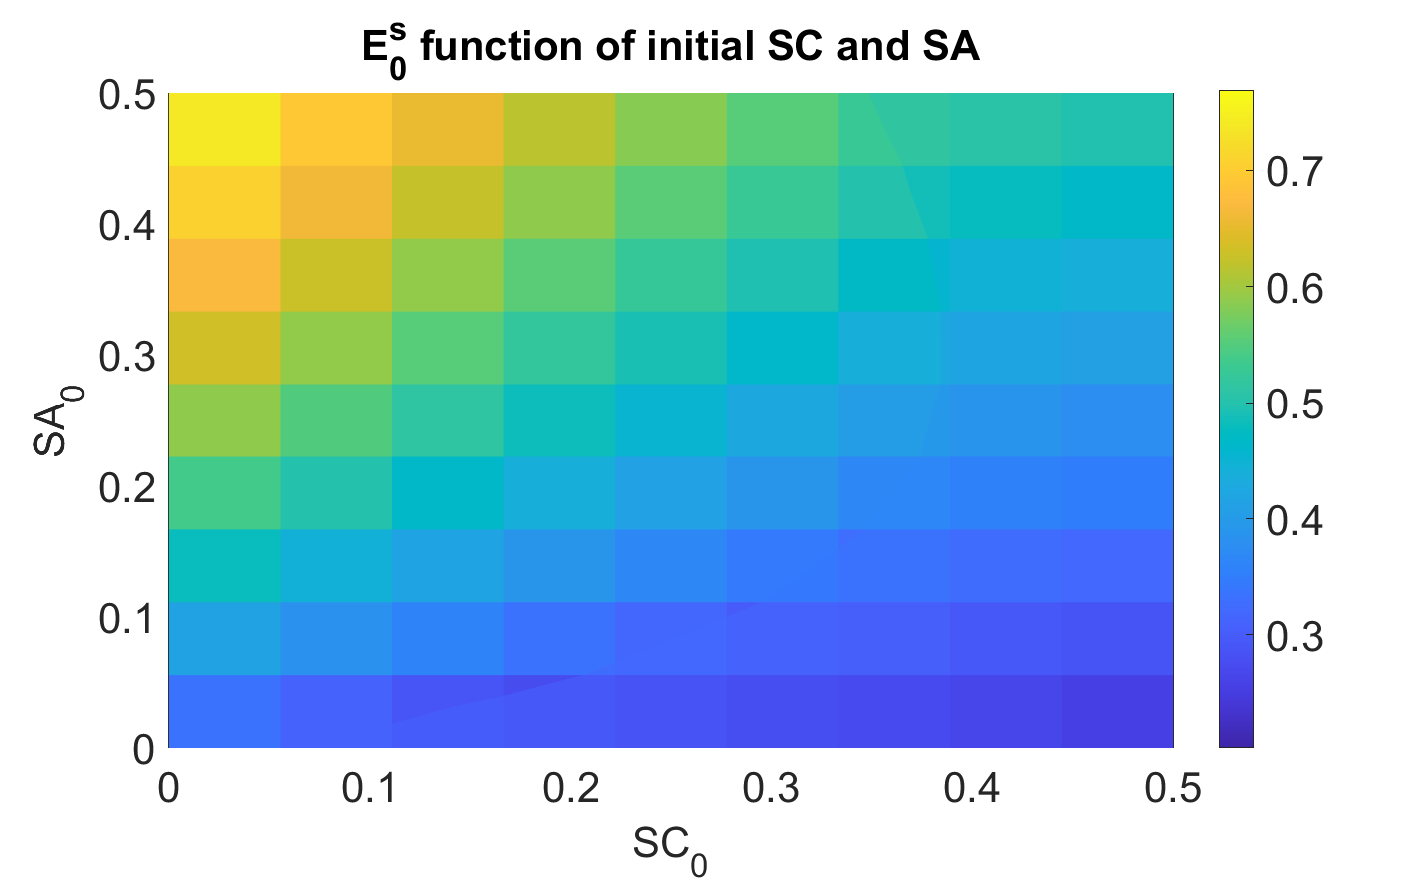
\includegraphics[width=0.48\linewidth]{1_corpo/figure/behav_epi_sim/HMap_SC0_SA0_B1_B2_equal}}\\
	\caption[Heat map full model first case]{Simulations of $E_0^s$ with $\mathcal{B}_1, \mathcal{B}_2 >1$, $\mathcal{B}_1 =  \mathcal{B}_2$, and $\lambda_1 < \lambda_2$.}
	\label{fig:Hmap_B1_B2_equal}
\end{figure}

\begin{figure}[h]
	\centering
	\subfloat[][\emph{$\rho$ and $SC_0$ dependence.}]
	{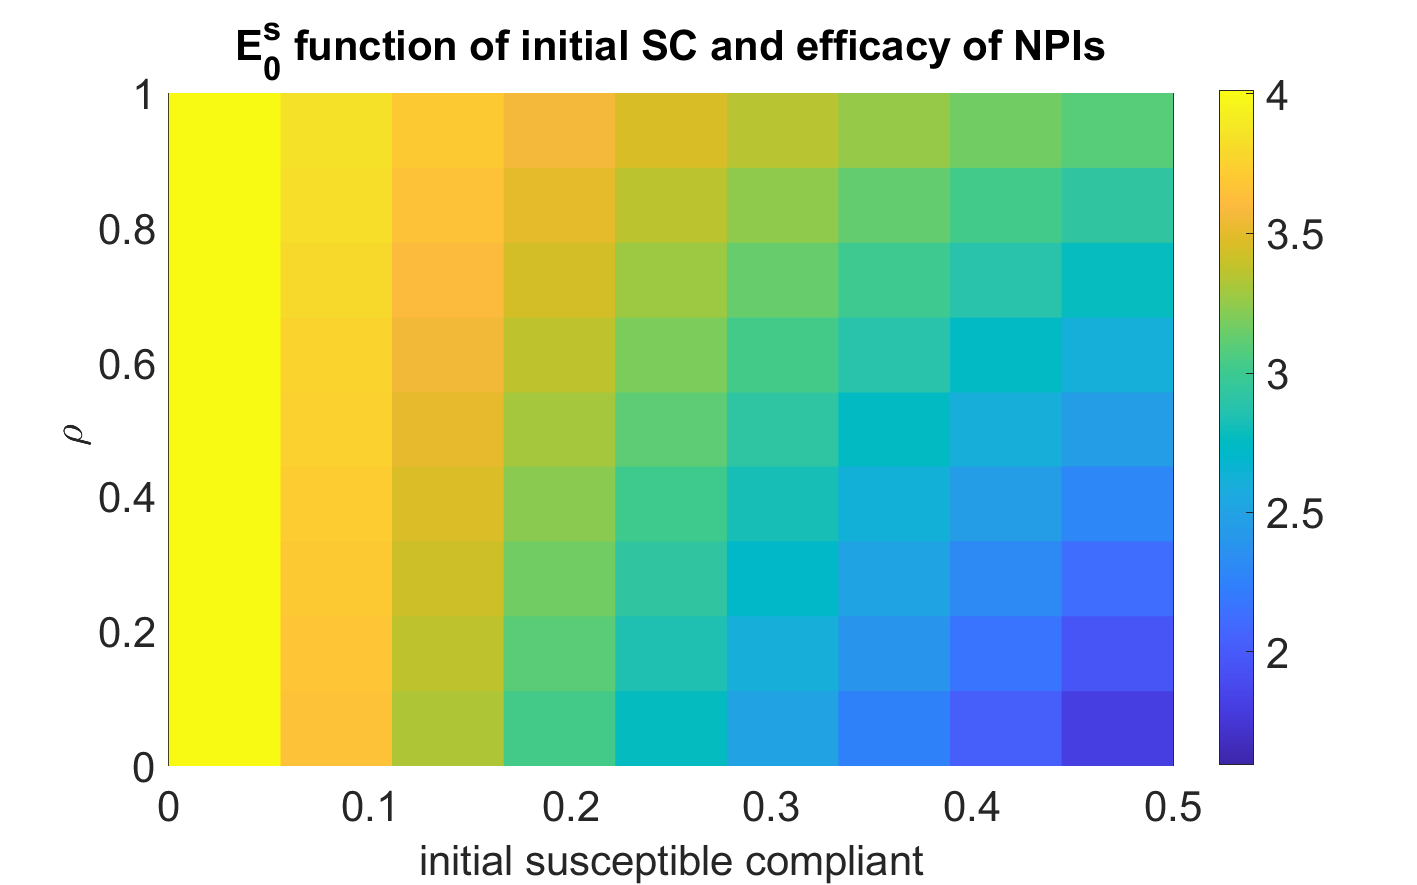
\includegraphics[width=0.48\linewidth]{1_corpo/figure/behav_epi_sim/HMap_SC0_rho_B1_mag_B2}} \quad
	\subfloat[][\emph{ $SA_0$ and $SC_0$ dependence.}]
	{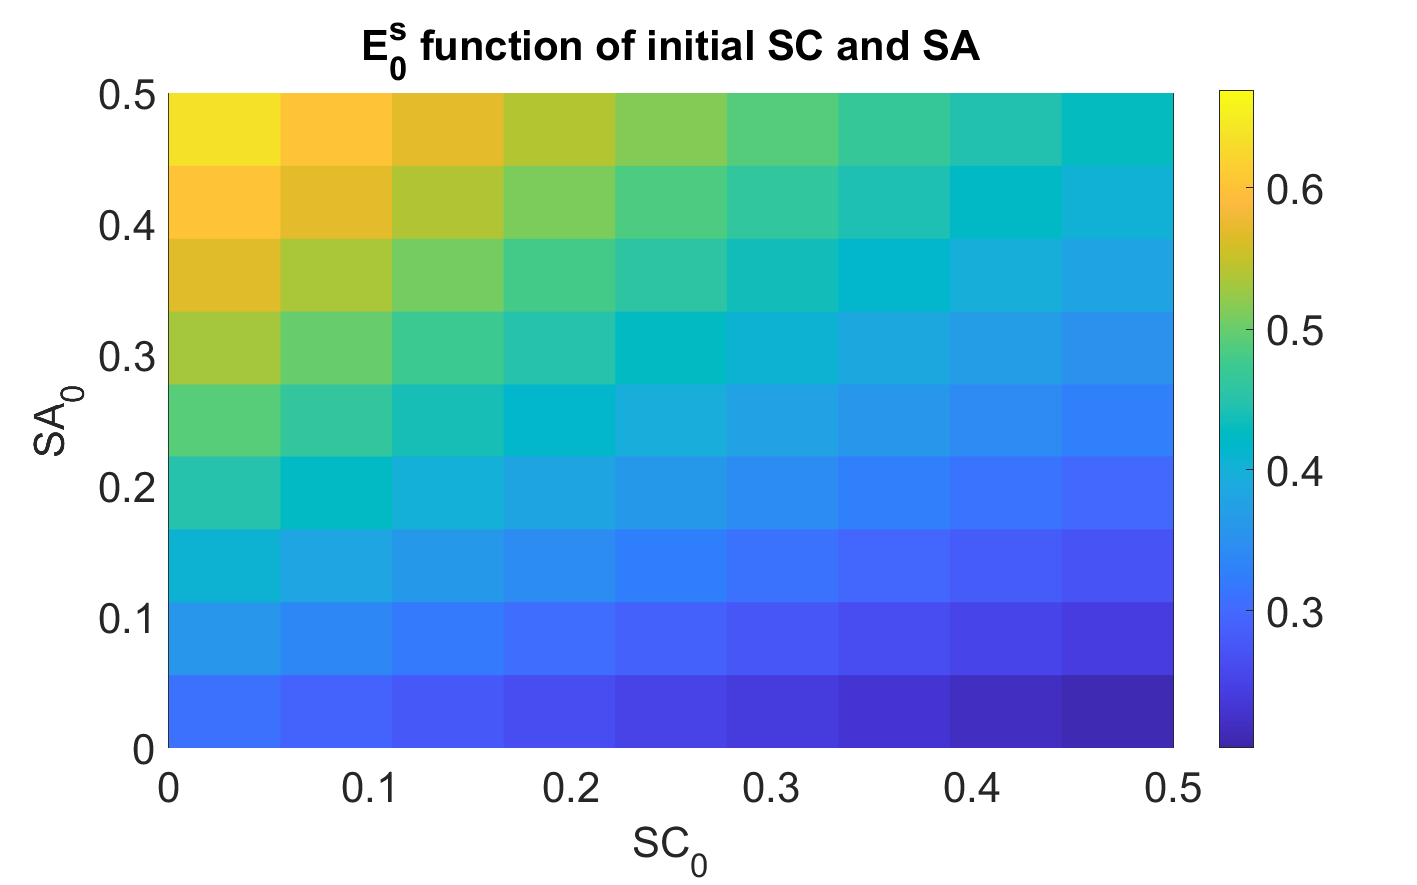
\includegraphics[width=0.48\linewidth]{1_corpo/figure/behav_epi_sim/HMap_SC0_SA0_B1_mag_B2}}\\
	\caption[Heat map full model first case]{Simulations of $E_0^s$ with $\mathcal{B}_1, \mathcal{B}_2 >1$, $\mathcal{B}_1 >  \mathcal{B}_2$, and $\lambda_1 = \lambda_2$.}
	\label{fig:Hmap_B2_less_B1}
\end{figure}

\begin{figure}[h]
	\centering
	\subfloat[][\emph{$\rho$ and $SC_0$ dependence.}]
	{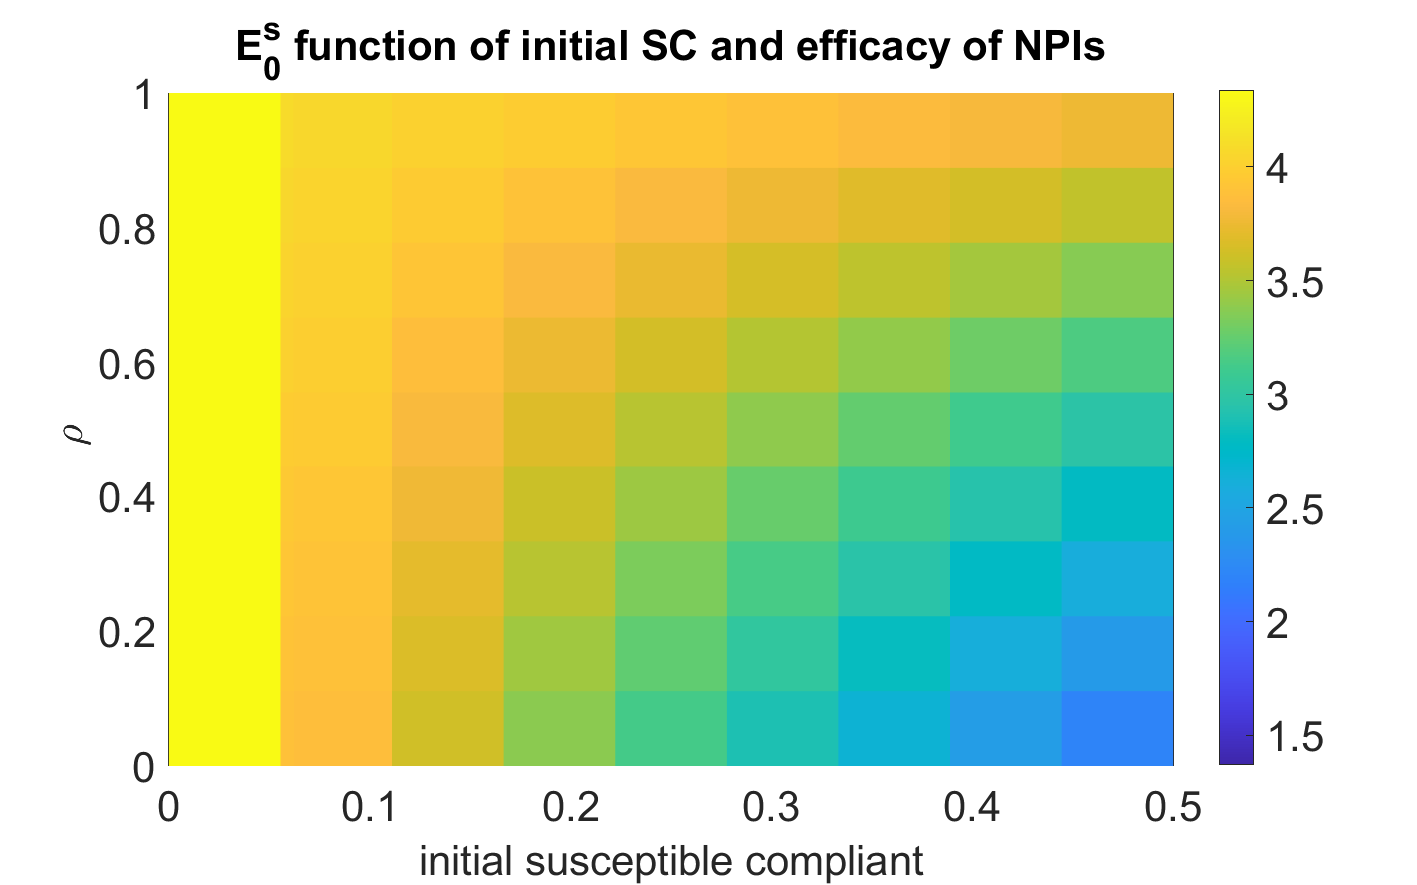
\includegraphics[width=0.48\linewidth]{1_corpo/figure/behav_epi_sim/HMap_SC0_rho_B1_mag_B2_lambda2_mag}} \quad
	\subfloat[][\emph{ $SA_0$ and $SC_0$ dependence.}]
	{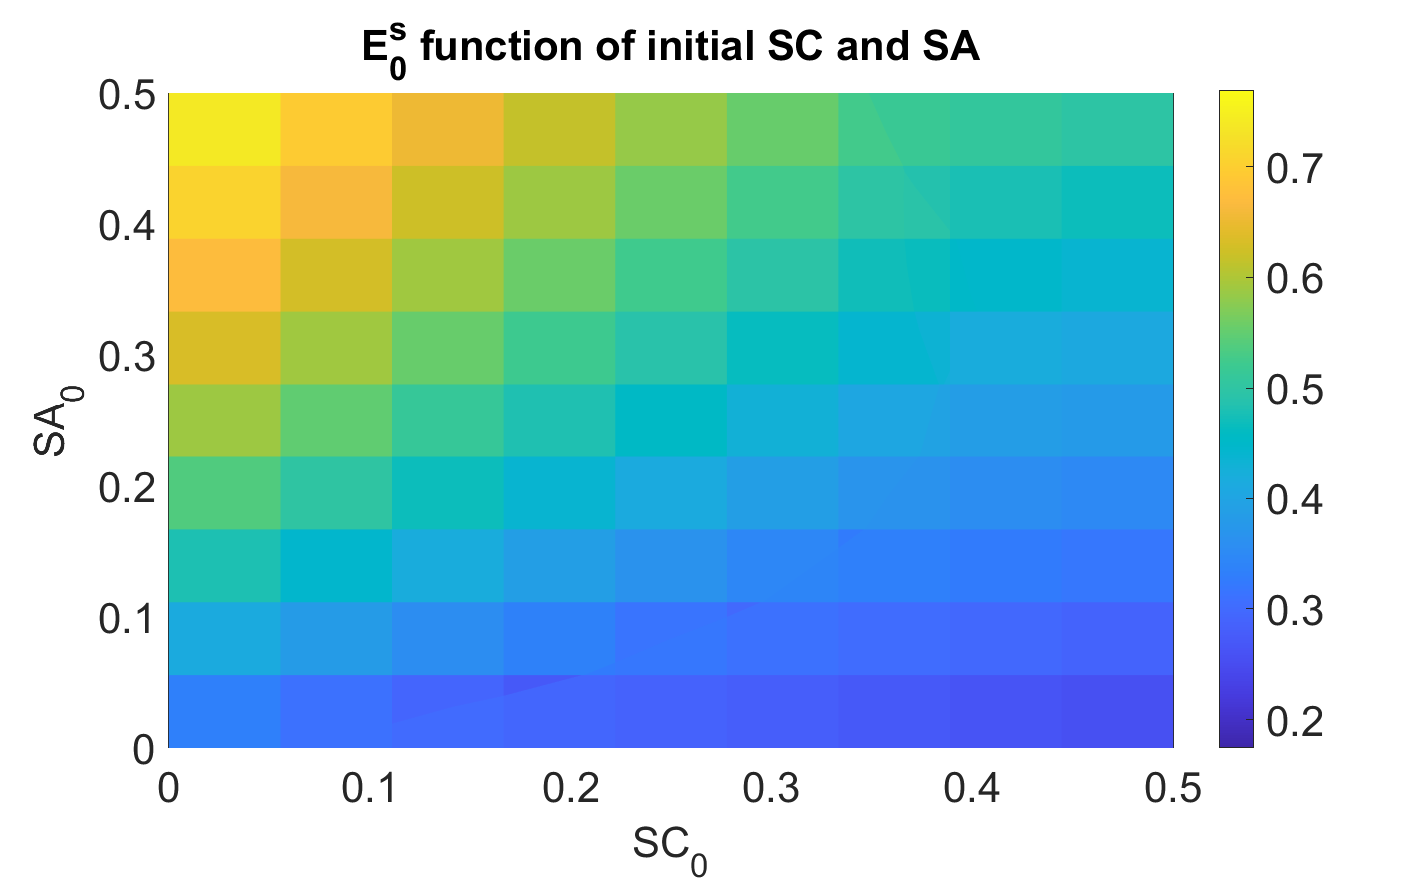
\includegraphics[width=0.48\linewidth]{1_corpo/figure/behav_epi_sim/HMap_SC0_SA0_B1_mag_B2_lambda2_mag}}\\
	\caption[Heat map full model first case]{Simulations of $E_0^s$ with $\mathcal{B}_1, \mathcal{B}_2 >1$, $\mathcal{B}_1 >  \mathcal{B}_2$, and $\lambda_1 < \lambda_2$.}
	\label{fig:Hmap_B2_less_B1_lam2}
\end{figure}